\documentclass{standalone}
\usepackage{tikz}
\usetikzlibrary{arrows,positioning,automata,shadows,fit,shapes}
\begin{document}
    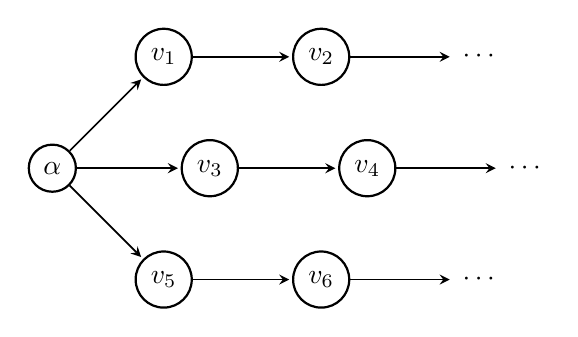
\begin{tikzpicture}[
            > = stealth, % arrow head style
            shorten > = 1pt, % don't touch arrow head to node
            auto,
            node distance = 2cm, % distance between nodes
            semithick % line style
        ]

        \tikzstyle{every state}=[
            draw = black,
            thick,
            fill = white,
            minimum size = 4mm
        ]

        \node[state] (s) {$\alpha$};
        \node[state] (v1) [above right of = s] {$v_1$};
        \node[state] (v2) [right of=v1] {$v_2$};
        \node[state] (v3) [right of=s] {$v_3$};
        \node[state] (v4) [ right of=v3] {$v_4$};
        \node[state] (v5) [below right of=s] {$v_5$};
        \node[state] (v6) [right of=v5] {$v_6$};
        \node (etc1) [right of=v2] {$\cdots$};
        \node (etc2) [right of=v4] {$\cdots$};
        \node (etc3) [right of=v6] {$\cdots$};


        \draw[->] (s) -- (v1);
        \draw[->] (v1) -- (v2);
        \draw[->] (s) -- (v3);
        \draw[->] (v3) -- (v4);
        \draw[->] (s) -- (v5);
        \draw[->] (v5) -- (v6);
        \draw[->] (v2) -- (etc1);
        \draw[->] (v4) -- (etc2);
        \draw[->] (v6) -- (etc3);

    \end{tikzpicture}
\end{document}
